\documentclass[12pt,a4paper]{article}
\usepackage[utf8]{inputenc}
\usepackage[T1]{fontenc}
\usepackage[francais]{babel}
\usepackage{amsmath}
\usepackage{amsfonts}
\usepackage{amssymb}
\usepackage{graphicx}
\usepackage[top=2.00cm]{geometry}
\usepackage{titlesec}
\usepackage{capt-of}
%%modif des titres de section diminuer la taille

\renewcommand{\thesection}{\Roman{section}}
\titleformat{\section}
{\normalfont\bfseries\Large\scshape}{\thesection}{1em}{}
\titleformat{\subsection}
{\normalfont\bfseries\large}{\thesubsection}{1em}{}

\makeatletter
\def\@maketitle{
	
	\begin{center}
		% NoLogo
		% \vspace*{+2cm}
		
		% Corner Logo
		% \begin{flushright}
		%  \includegraphics[width=40mm]{logo_corner}\\[4ex]
		% \end{flushright}
		
		% Top Logo
		\includegraphics[scale=0.3]{res/logo_top}
		
		
		{\LARGE \@title }\\[4ex]
		{\large \@author}\\[4ex]
		{\large \@date}\\[8ex]
		\rule{\linewidth}{0.4pt}
	\end{center}
}
\makeatletter

\author{CHARNAY Valentin, FINOT Sylvain}
\title{Compte rendu de TP :\\[4pt] \scshape Photodétecteurs}

\date{\today}
\begin{document}
	\maketitle
	Le but de ce TP est d'étudier le comportement (la réponse) de différents photodétecteurs en fonction de différents paramètres. Nous étudierons :
	\begin{itemize}
		\item La réponse en fonction du flux lumineux
		\item La réponse spectrale (i.e en fonction de la longueur d'onde)
		\item La réponse temporelle
	\end{itemize}
	
	\section{La photorésistance}
	\subsection{Réponse en fonction du flux}
	Pour effectuer cette étude correctement, il faut connaitre le flux théorique reçu par le détecteur.
	On utilise deux polariseurs, le premier pour but de polariser la lumière, on a alors une lumière d'intensité $I_0$ polariser. Le deuxième polariseur que l'on vient accoler au premier sert alors a contrôler l'intensité lumineuse par la loi de Malus:
	$$I=I_0\cos^2(\theta)$$
	Le flux est donc proportionnel à cette quantité. En réalité on tracera nos graphs en fonction de $\dfrac{I}{I_0}=\cos^2(\theta)$\\
	\textbf{Remarque :} Il suffit de faire le relevé de la réponse uniquement pour $\theta \in \left[0,\dfrac{\pi}{2} \right]$
	
	Dans un premier temps, nous avions aligné les polariseurs sur leur 0 respectif, cependant cela ne correspondait pas à un maximum du flux lumineux. En réalité il y avait un décalage de 305$^{\circ}$.
	Pour aligner/étalonner les polariseurs, on les superpose et on cherche la position pour laquelle l'intensité lumineuse est nulle, cela signifie qu'il y a un écart de 90$^\circ$.\\
	Nous avons fait une partie des mesures sans avoir corrigé le décalage. Pour retrouver le bon angle entre les deux polariseurs, cela revient à faire un changement d'origine.
	$$\theta \rightarrow \theta -305^{\circ} +360^{\circ}$$
	On ajoute 360 pour retrouver une valeur dans $\left[0,360\right]$
	
	En effectuant les relevés on obtient : 
	\begin{center}
		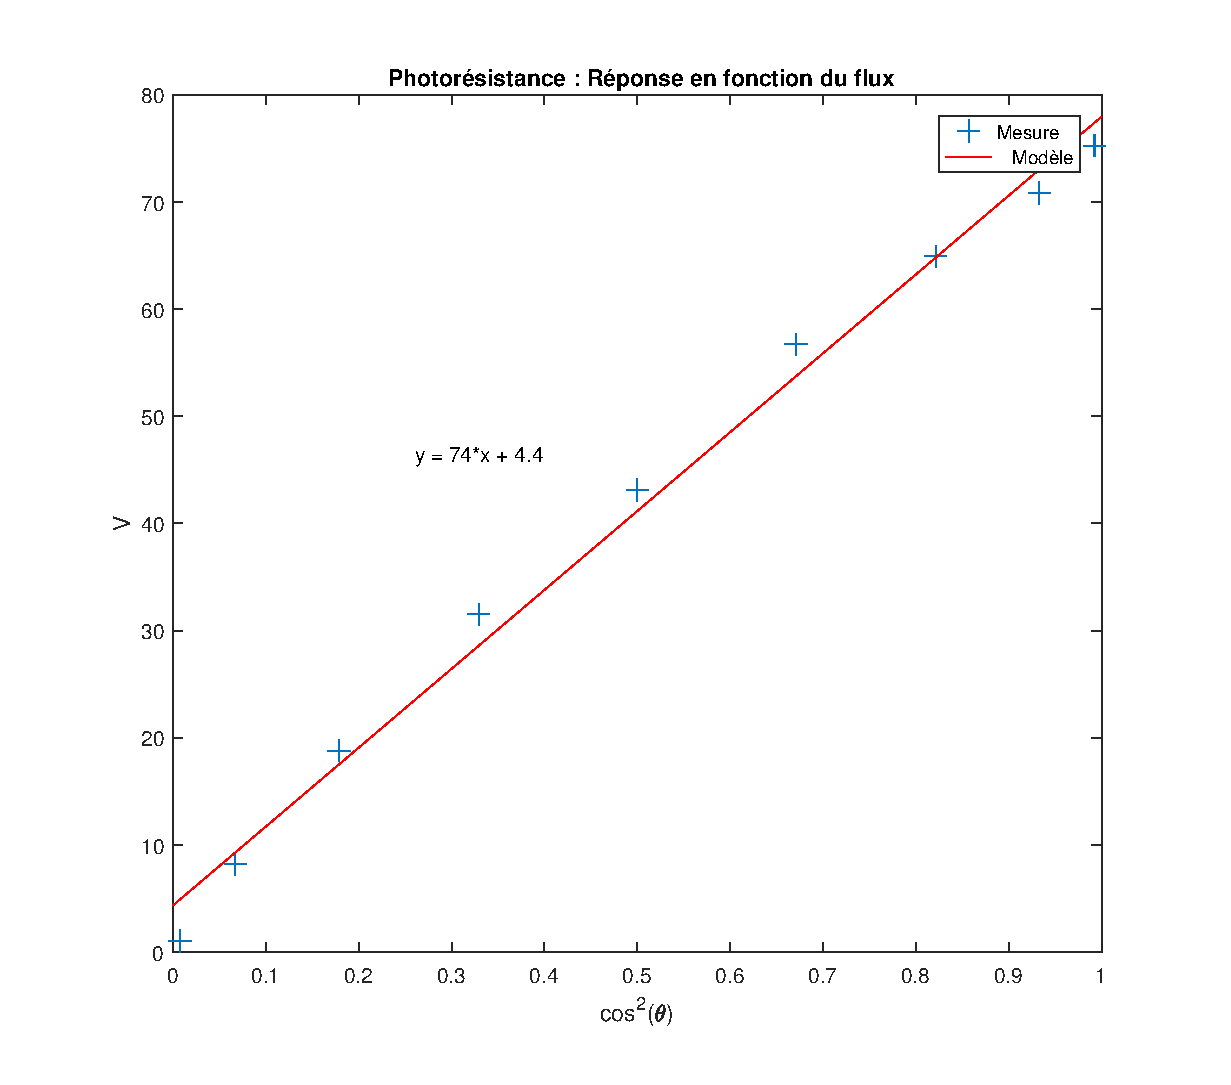
\includegraphics[width=0.8\linewidth]{res/photoresistance_flux.eps}
	\end{center}
	Le modèle linéaire semble correspondre relativement bien à la réponse de la photorésistance.
	
	\subsection{Réponse spectrale}
	Pour étudier la réponse spectrale, on utilise un monochromateur.
	On peut alors mesurer la réponse de la photorésistance en fonction de la longueur d'onde $\lambda$
	\begin{center}
		\includegraphics[scale=0.7]{res/photoresistance_spectrale.eps}
	\end{center}
	Cette courbe nous montre que la réponse de la photorésistance est maximale pour une longueur d'onde donnée (ici 600nm).
	
	\subsection{Réponse temporelle}
	Nous avons essayé d'étudier la réponse temporelle de la photorésistance, cependant nous n'avons pas trouvé de signal sur l'oscilloscope. Il se pourrait que la photorésistance ait une réponse temporelle très médiocre.
	
	\section{La photodiode}
	\subsection{Réponse en fonction du flux}
	En traçant la courbe grossièrement, on se rend compte que la réponse de la diode n'est pas linéaire. En supposant que la réponse s'exprime sous la forme : $$V(\Phi)=\alpha\Phi^{\beta}$$
	On trace $\ln(V)=f(\ln(\Phi))$.\\
	En réalité on trace en fonction de $\dfrac{I}{I_0}=\cos^2(\theta)$. Le flux est proportionnel à cette quantité.\\
	On remarque alors que le résultat peut s'approximer par un modèle affine ayant pour coefficients:\\
	\begin{center}
		\begin{tabular}{ll}
			K & 0.06742\\
			C & -0.6535\\
		\end{tabular}
	\end{center}
	\begin{align*}
	V(\Phi) &=\alpha\Phi^{\beta}\\
	\iff \ln(V) &=\ln(\alpha\Phi^{\beta})\\
	&=\beta\ln(\Phi)+\ln(\alpha)\\[2em]
	%
	\implies \alpha &=\exp(C)=0,52\\
	\beta &= K=0,067
	\end{align*}
	\begin{center}
		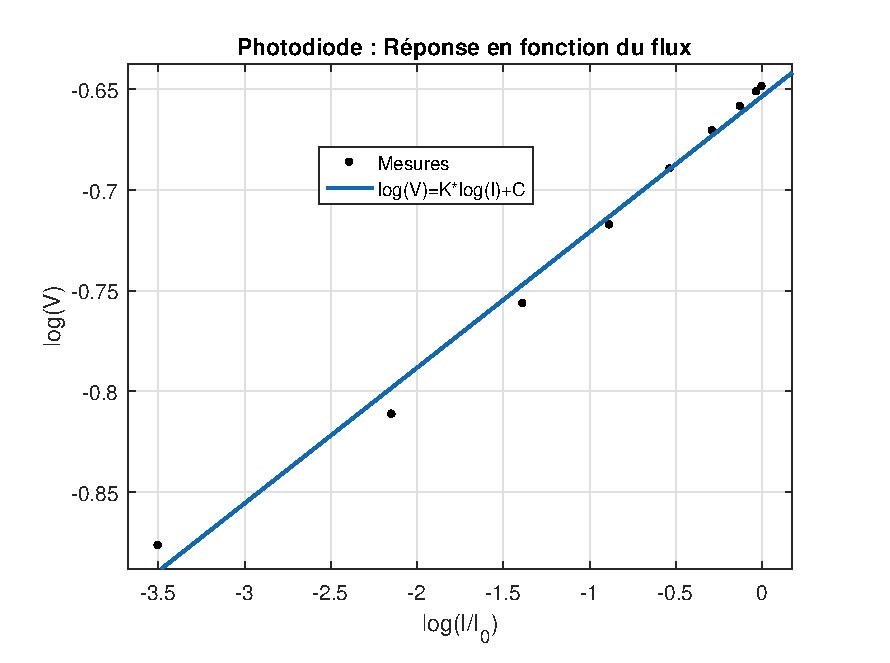
\includegraphics[width=0.8\linewidth]{res/diode_flux.eps}
	\end{center}
	\subsection{Réponse spectrale}
	On utilise la même technique que précédemment.\\
	On obtient cette fois-ci le graphe suivant :\\
	On remarque là aussi qu'il y a un maximum pour $\lambda\approx600$nm. Cependant, contrairement à la photorésistance, la différence entre la réponse maximale et minimale est moins importante.\\
	Nous avons pris des points pour $\lambda \in \left[450,800\right]$, après réflexion, nous  aurions pu prendre quelques points supplémentaires à la frontière entre visible et ultraviolets.\\
	En observant le graphique, il semblerait que la photodiode soit plus sensible aux basses longueurs d'onde que la photorésistance.
	\begin{center}
		\includegraphics[scale=0.8]{res/photodiode_spectrale.eps}
	\end{center}
	\subsection{Réponse temporelle}
	En alimentant un laser avec un signal créneau (généré avec un générateur basse fréquence), on essaye de retrouver les créneaux avec la photodiode.
	
	
	La première photodiode que nous avons utilisée ne donnait pas de résultats concluants.
	Nous en avons donc changé pour une de meilleure qualité (photodiode avalanche).\\
	La réponse était fidèle au signal d'entrée pour un signal allant jusqu'au kHz.
	En dépassant le kHz, on observe des déformations.  
	\begin{figure}[h]
		\centering
		\includegraphics[width=0.7\linewidth]{"res/7,2kHz 50us"}
		% \caption[7,2kHz]{}
		\caption{Entrée et réponse à 7,2kHz}
		\label{fig:72khz-50us}
	\end{figure}
	On détecte toujours des impulsions, mais la diode a du retard, on n'observe plus la même fréquence.
	
	En augmentant grandement la fréquence, la réponse de la diode devient une sinusoïde. Certes, on ne détecte plus la forme de l'impulsion, mais on détecte toujours l'impulsion à une fréquence relativement élevée pour une diode (ici $\approx$30kHz). 
	\begin{center}
		\includegraphics[width=0.7\linewidth]{res/20170308_165725}
		\captionof{figure}{Réponse temporelle à environ 30kHz}
	\end{center}
	\section{La thermopile}
	\subsection{Réponse en fonction du flux}
	En faisant le relevé, il semblerait que la réponse de la thermopile soit linéaire% à partir d'un certain seuil. En regardant le graph ci dessous, on remarque qu'on n'arrive pas a détecter de flux pour $\theta \in \left[90,100\right]$.
	\begin{center}
		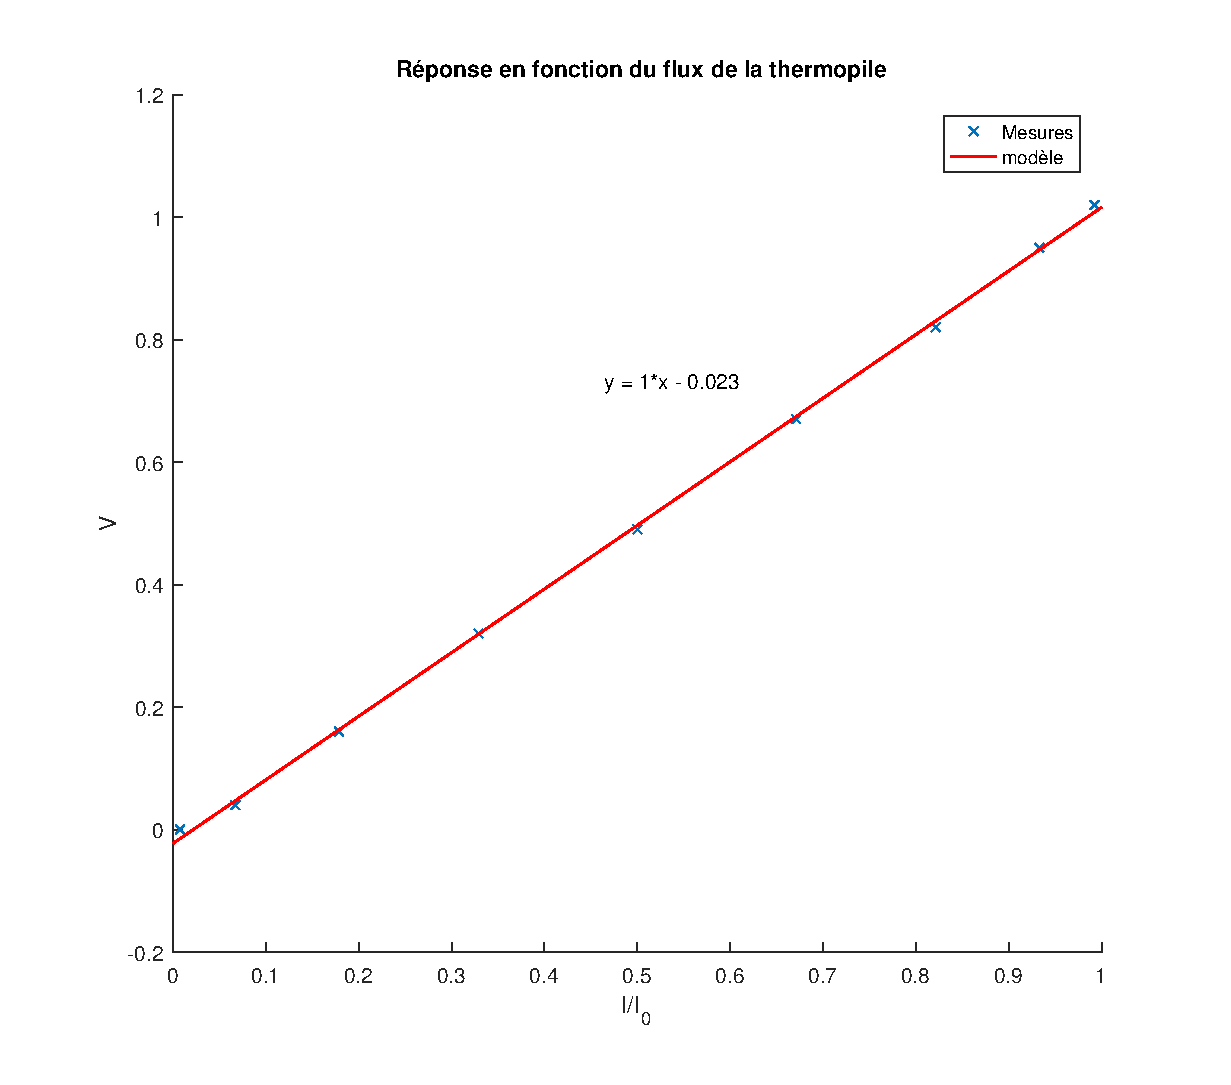
\includegraphics[width=0.7\linewidth]{res/thermopile_flux}
	\end{center}
\end{document}

